\chapter{It\^o Stochastic Calculus}
\label{ch:ItoCalc}
In this section we will give the idea behind the construction of the stochastic integral in the It\^o-sense for a certain class of functions \(\mathcal{C}\).
We will also present the fundamental theorem of stochastic calculus, namely \emph{It\^o's lemma}, and give examples. Later we will discuss an important application of this lemma, the so-called \emph{stochastic Taylor expansion} (or \emph{Wagner-Platen expansion}). We will use it to construct our numerical schemes which we will discuss in chapter \ref{ch:Num}.
\section{Construction of the It\^o stochastic integral}
We want to define:
\[\int_0^T \! X_t \, \mathrm{d}W_{t}\]
for a large class of functions \(X_t\in\mathcal{C}(0,T)\), \(X_t\!:[0,T]\!\times\Omega\rightarrow\mathbb{R}\).

First let us define the space of square-integrable stochastic processes:
\[L^{2}[0,T] \coloneqq \{X_t\!: [0,T]\times\Omega \rightarrow \mathbb{R}\mid X_t \text{ measurable},\, \mathbb{E}[\int^{T}_{0}X_t^2\mathrm{d}t]<\infty\}.\]
If we interpret the second condition as norm, we get the \emph{complete normed space} \((L^{2}[0,T], \|\cdot\|_{L^2[0,T]})\).
However we want to exclude functions from this class which are not \(\mathcal{F}_t\)-adapted.
Let us consider now the subset \(\mathcal{C}\coloneqq\mathcal{C}[0,T]\) of all functions \(X_t\) in \(L^{2}[0,T]\) which are adapted.
A limit of a sequence of adapted processes remains adapted\footnote{See \cite{BMKaratzas} for the proof.}. Thus \(\mathcal{C}\) is a closed subset of \(L^2[0,T]\) since it includes all its limits, which implies that \(\mathcal{C}\) is also complete under the same norm. Thus we have the complete normed space \((\mathcal{C}, \|\cdot\|_{L^2[0,T]})\). Recall that we want to define the It\^o stochastic integral for functions in \(\mathcal{C}\). 
First we will define the stochastic integral for a simpler class of functions \(\mathcal{E}\), s.t \(\mathcal{E}\subset\mathcal{C}\), and then expand the definition to the space \(\mathcal{C}\).

Define the space of \emph{random step functions} \(\mathcal{E}\) which can be expressed in the following form:
\[\xi_t^{n} = \sum^{n-1}_{k=0}Z_k\cdot\mathbb{1}_{[t_k,t_{k+1})}\]
for a partition \(P_n\) of [0,T] and some random variables \(Z_k \:\:\mathcal{F}_{t_k}\)-measurable and square-integrable (this means \(Z_k\) is in \(L_2[\Omega]\)) for \(k\!=\!0,\dots,\! n\!-\!1\).
Obviously \(\xi_t^{n}\) is \(\mathcal{F}_t\)-adapted and \(\mathcal{E}\subset\mathcal{C}\).
\begin{definition}[It\^o stochastic integral for random step functions]
Let \(\xi_t^{n}\!\in\mathcal{E}\) be a random step function with the above representation. Then 
\begin{displaymath}
\int_0^T \! \xi_t^{n}\, \mathrm{d}W_{t}\coloneqq\sum^{n-1}_{k=0}Z_k\cdot(W_{t_{k+1}}-W_{t_{k}})
\end{displaymath}
is the It\^o stochastic integral of \(\xi_t^{n}\). Note that the integral is a random variable and \(\mathcal{F}_T\)-measurable. If we allow the upper limit of the integral to be in the intervall [0,T], then the It\^o stochastic integral becomes an adapted
stochastic process. This would not be true in the Stratonovich calculus or if \(X_t\) were not adapted.
\end{definition}
For \(X_t\in\mathcal{C}\) we have the construction \(\xi_t^{n}=\sum^{n-1}_{k=0}X_{t_k}\cdot\mathbb{1}_{[t_k,t_{k+1})}\) which is also adapted. 

\begin{figure}[!h]
\centering
  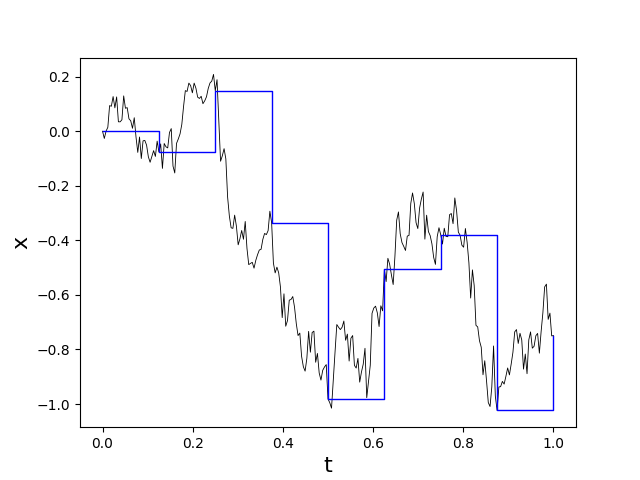
\includegraphics[scale=0.6]{content/Graphics/Figure_WienerStepProcess.png}
  \caption{A sample of the Wiener process and its corresponding step function  for n = 8.}
  \label{fig:fig3}
\nopagebreak
\end{figure}	
The following result will be important for our construction of It\^o stochastic integrals for functions in \(\mathcal{C}\):
\begin{proposition}[It\^o-isometry for random step functions]
Let \(\xi_t\!\in\mathcal{E}\). Then
\begin{align*}
\mathbb{E}[(\int_0^T\!\xi_t\,\mathrm{d}W_{t})^2] = \mathbb{E}[\int_0^T\!(\xi_t)^2\,\mathrm{d}t]\\
\|\int_0^T\!\xi_t\,\mathrm{d}W_{t}\|_{L^2[\Omega]} = \|\xi_t\|_{L^2[0,T]}.
\end{align*}
We conclude that for all \(\xi_t\in\mathcal{E}\) there exists \(\int_0^T\!\xi_t\,\mathrm{d}W_{t}\) as an element in \({L^2[\Omega]}\).
\end{proposition}
\begin{proof}
\begin{flalign*}
& \mathbb{E}[(\int_0^T\!\xi_t\,\mathrm{d}W_{t})^2]  \\
&= \mathbb{E}[(\sum^{n-1}_{k=0}Z_k\cdot(W_{t_{k+1}}-W_{t_{k}}))(\sum^{n-1}_{l=0}Z_l\cdot(W_{t_{l+1}}-W_{t_{l}}))] \\
&= \mathbb{E}[\sum^{n-1}_{k=0}Z_k^2\cdot(W_{t_{k+1}}-W_{t_{k}})^2] + 2\mathbb{E}[\sum^{n-1}_{k>l=0}Z_k\cdot Z_l\cdot(W_{t_{k+1}}-W_{t_{k}})(W_{t_{l+1}}-W_{t_{l}})] \\
&= \sum^{n-1}_{k=0}\mathbb{E}[Z_k^2]\cdot\mathbb{E}[(W_{t_{k+1}}-W_{t_{k}})^2]\\
& \text{Where we used that \(Z_k^2\), \((W_{t_{k+1}}-W_{t_{k}})^2\)  and \(Z_l\cdot(W_{t_{k+1}}-W_{t_{k}})(W_{t_{l+1}}-W_{t_{l}})\), \(Z_k\)}\\
& \text{are independent for } k>l. \\
& \sum^{n-1}_{k=0}\mathbb{E}[Z_k^2]\cdot(t_{k+1}-t_{k}) = \mathbb{E}[\int_0^T\!(\xi_t)^2\,\mathrm{d}t]
\end{flalign*}
\end{proof}
The proof would not be possible in case of the Stratonovich calculus or if \(X_t\) were not adapted. For example if \(X_t = W_{t+\frac{1}{2}}\).

Finally, using the following lemma, we can expand our definition of the stochastic integral from \(\mathcal{E}\) to \(\mathcal{C}\):
\begin{lemma}[It\^o stochastic integral]
Let \(X_t\in\mathcal{C}\). Then there exists a sequence \(({\xi_{t}^n})_{n\!\in\!\mathbb{N}}\in\mathcal{E}\) s.t.
\(\mathbb{E}[\int_{0}^{T}(X_t-\xi_{t}^n)^2\mathrm{d}t] = \|X_t-\xi_{t}^n\|^2_{L^2[0,T]}\rightarrow 0\:\text{as}\:n\rightarrow\infty\) and 
\begin{align*}
\int_{0}^{T}\xi_t^n\mathrm{d}W_t\rightarrow\int_{0}^{T}X_t\mathrm{d}W_t\quad(\text{in}\:L^2[\Omega])\:\:\text{as}\:n\rightarrow\infty.
\end{align*}
This means \(\|\int_{0}^{T}X_t\mathrm{d}W_t-\int_{0}^{T}\xi_t^n\mathrm{d}W_t\|_{L^2[\Omega]} \rightarrow 0\:\:\text{as}\:n\rightarrow\infty.\)
And we can define:
\[\int_0^T\! X_t\,\mathrm{d}W_{t} \coloneqq\lim_{n\to\infty}\int_0^T\! \xi_t^n\,\mathrm{d}W_{t}  \:\:(\text{in}\:L^2[\Omega]).\]
Additionaly, the It\^o-isometry holds also in \(\mathcal{C}\).
\end{lemma}

The idea of the construction is to show that \(\mathcal{E}\) is dense in \(\mathcal{C}\) w.r.t the norm \(\|\cdot\|_{L^2[0,T]}\) using an approximation procedure, see \cite{Oksendal} for the details.
This means there exists a sequence \((\xi_t^n)_{n\!\in\!\mathbb{N}}\in\mathcal{E} \text{ s.t. } \|X_t-\xi_t^n\|_{L^2[0,T]}\rightarrow 0 \text{ as } n\rightarrow\infty\:\:\forall\: X_t\in\mathcal{C}\).
Since \( L^2[0,T]\) is complete, \(({\xi_t^n})_{n\!\in\!\mathbb{N}}\) is a Cauchy-sequence in this space. Using the It\^o-isometry, we then have:
\[\|\xi_t^n-\xi_t^m\|_{L^2[0,T]} = \|\int_{0}^{T}\xi_t^n\mathrm{d}W_t-\int_{0}^{T}\xi_t^m\mathrm{d}W_t\|_{L^2[\Omega]}\rightarrow 0 \text{ as } n,m\rightarrow\infty.\]
Hence \(({\int_{0}^{T}\xi_t^n}\mathrm{d}W_t)_{n\!\in\!\mathbb{N}}\) is a Cauchy-sequence in \(L^2[\Omega]\). It is well known that this space is complete\footnote{\(L^2[\Omega]\) is the usual space of square-integrable random variables on
\(\left( \Omega , \mathcal{F}, P\right)\).}. 
Thus, it makes sense to define:
\[\int_0^T\! X_t\,\mathrm{d}W_{t} \coloneqq\lim_{n\to\infty}\int_0^T\! \xi_t^n\,\mathrm{d}W_{t} \quad(\text{in }L^2[\Omega])\]
as an element in \(L^2[\Omega]\).

 
We still need to clarify why we choose It\^o over Stratonovich. As can be seen, the definition due to It\^o simplifies our calculations and enables us to define the stochastic integral in a straightforward way through the isometry. The isometry does not hold in the Stratonovich calculus. Additionaly we are able to identify the It\^o stochastic integral as a martingale\footnote{See \cite{Oksendal} for the interpretation of It\^o stochastic integrals as martingales. The expected value of the It\^o stochastic integral is always 0 and the It\^o stochastic integral can be defined as adapted stochastic process.}.


\section{Lemma of It\^o}
\label{itolemma}
The lemma of It\^o enables us to evaluate stochastic integrals without using the definition as in section \ref{lemma:StochInt}. 
Given a stochastic process \(X_t\) and its representation as stochastic integral equation, we may ask, what is the representation of \(u(X_t)\) where u:\(\mathbb{R}\to\mathbb{R}\) is a smooth map? 
We will present the lemma of It\^o in 3 cases: In the first case, \(X_t=W_t\) and we are interested in \(u(W_t)\). Then we will consider more general stochastic processes \(X_t\). Finally we will allow the mapping u:\(\mathbb{R}\times[0,T]\to\mathbb{R}\) to depend on the paramter t.
\begin{definition}[It\^o process]
\label{Itoprocess}
We will call a stochastic process \(X_t\) an It\^o process if it has a known representation as stochastic integral equation of the following form:
\[X_t - X_0 = \int_0^t \!a(X_s,s)\,\mathrm{d}s + \int_0^t \!b(X_s,s)\,\mathrm{d}W_{s}\]
where \(b(X_t,t)\in\mathcal{C},\:\: a(X_t,t)\: \mathcal{F}_t\)-adapted and \(\mathbb{E}[\int_{0}^{T}(a(X_t,t))^2\mathrm{d}t]<\infty\). \\
Then \(X_t\in L_2[\Omega]\) \(\forall\; t\in[0,T]\) fixed and we have the (symbolical) differential form:
\[\mathrm{d}X_t = a(X_t,t)\mathrm{d}t + b(X_t,t)\mathrm{d}W_t.\]
We will only consider the autonomous case where the functions \(a(x,t) \equiv a(x)\) and \(b(x,t) \equiv b(x)\) do not depend on the additional parameter t.

\end{definition}
\begin{lemma}[It\^o lemma for the Wiener process]
Let \(W_t\) be the Wiener process. Let u:\(\mathbb{R}\to\mathbb{R}\) be twice continuously differentiable with derivatives \(u_x(x), u_{xx}(x)\). Define \(Y_t \coloneqq u(W_t)\). Then
\begin{displaymath}
Y_t-Y_0 = \int_0^t \!\frac{1}{2}u_{xx}(W_s)\,\mathrm{d}s + \int_0^t \!u_x(W_s)\,\mathrm{d}W_{s}
\end{displaymath}
where equality is P-a.s. for \(t\in[0,T]\).
\end{lemma}
\begin{proof}
Proof follows from the general case, lemma \ref{lemma:ito}, and by using that \(W_t = \int_0^t \!\,\mathrm{d}W_{s}\).
\end{proof}
\begin{lemma}[It\^o lemma, non time-dependent case]
Let \(X_t\) be an It\^o process. 
Let u:\(\mathbb{R}\to\mathbb{R}\) be twice continuously differentiable with derivatives \(u_x(x), u_{xx}(x)\). Define \(Y_t \coloneqq u(X_t)\). Then
\begin{displaymath}
Y_t-Y_0  = \int_0^t \!u_x(X_s)a(X_s) + \frac{1}{2}u_{xx}(X_s)b(X_s)^2\,\mathrm{d}s + \int_0^t \!u_x(X_s)b(X_s)\,\mathrm{d}W_{s} 
\end{displaymath}
where equality is P-a.s. for \(t\in[0,T]\).
\end{lemma}
\begin{proof}
See general case.
\end{proof}
\begin{lemma}[It\^o lemma, general case]
\label{lemma:ito}
Let \(X_t\) be an It\^o process. 
Let u:\(\mathbb{R}\times[0,T]\to\mathbb{R}\) be twice continuously differentiable with partial derivatives \(u_x(x,t), u_{xx}(x,t)\) and \(u_t(x,t)\). Define \(Y_t \coloneqq u(X_t,t)\).  Then
\begin{flalign*}
Y_t-Y_0  = & \int_0^t \!u_t(X_s,s)+u_x(X_s,s)a(X_s)\:\: + \\
		    & \frac{1}{2}u_{xx}(X_s,s)b(X_s)^2\,\mathrm{d}s + \int_0^t \!u_x(X_s,s)b(X_s)\,\mathrm{d}W_{s} 
\end{flalign*}
where equality is P-a.s. for \(t\in[0,T]\).
\end{lemma}
\begin{proof}
See \cite{Oksendal}.
\end{proof}
Let us consider some examples:
\begin{example}
Let \(X_t=W_t\) and u: \(x\mapsto x^2\). Then
\begin{flalign*}
& W_t^2 = \int_0^t \!\,\mathrm{d}s + \int_0^t \!2W_s\,\mathrm{d}W_{s}\\
& W_t^2 - t =  \int_0^t \!2W_s\,\mathrm{d}W_{s}\quad\text{by rearrangement.}
\end{flalign*}
This is the same result as in lemma \ref{lemma:StochInt} where we used the definition to calculate this stochastic integral in the It\^o sense.
\end{example}

\begin{example}
\label{ex:gbm}
Let \(X_t - X_0 = \int_0^t \!\mu X_s\,\mathrm{d}s + \int_0^t \!\sigma X_s\,\mathrm{d}W_{s}\). \(\mu,\:\sigma>0\) constants\\
and u: \(x\mapsto\ln(x)\: (x\neq 0)\). Then
\begin{flalign*}
& u_x(x) = \frac{1}{x}\:\:\text{ and }\:\:u_{xx}(x) = -\frac{1}{x^2} \\
u(X_t)-u(X_0) & = \int_0^t \!u_x(X_s)\mu X_s + \frac{1}{2}u_{xx}(X_s)(\sigma X_s)^2\,\mathrm{d}s + \int_0^t \!u_x(X_s)\sigma X_s\,\mathrm{d}W_{s} \\
			  & = \int_0^t \!\mu - \frac{1}{2}\sigma^2\,\mathrm{d}s + \int_0^t \!\sigma\,\mathrm{d}W_{s} = (\mu - \frac{1}{2}\sigma^2)t + \sigma W_t.\\
\end{flalign*}
This just means: 
\[\ln{X_t} = \ln{X_0} + (\mu - \frac{1}{2}\sigma^2)t + \sigma W_t\]
where \(X_0\) can be set as an initial value (can be a random variable under some conditions).
This example will be of importance in the next chapter.
\end{example}
\section{Stochastic Taylor expansions}
 \label{stochasticTaylor}

Given a deterministic and smooth function \(X(t)\) and \(\frac{\mathrm{d}}{\mathrm{d}t}X(t) = a(X(t))\) we can express it using the fundamental theorem of calculus as:
\[X(t)-X(0) = \int_0^t \!a(X(s))\,\mathrm{d}s.\]
We can reapply the theorem on \(a(X(s))\) and use the chain rule to get:
\begin{flalign*}
X(t)-X(0) & = \int_0^t \!a(X(0))\,\:+\,\:\int_0^s \!a^{\prime}(X(r))\cdot a(X(r))\,\mathrm{d}r\,\mathrm{d}s\\
		 & = a(X(0))t\,\:+\int_0^t\!\int_0^s \!a^{\prime}(X(r))\cdot a(X(r))\,\mathrm{d}r\,\mathrm{d}s.
\end{flalign*}
Indeed we could show this representation using the Taylor expansion and by plugging in the derivative of \(X(t)\).

The second integral is of quadratic order (\(\mathcal{O}(t^2)\)) (Where we assumed that the derivatives are bounded). If we truncate the second integral we can give a linear approximation of X(t) for t small, where \(x_0=X(0)\) is a given initial value.
This is the simplest approximation for (deterministic) ordinary differential equations, the so-called \emph{explicit Euler-scheme}.

We want to construct similar approximation schemes in the stochastic setting.
Let \(X_t\) be a stochastic process and its representation as It\^o process, where a:\(\mathbb{R}\to\mathbb{R}\), b:\(\mathbb{R}\to\mathbb{R}\) are smooth and have bounded derivatives (see \ref{Itoprocess}):
\[X_t - X_0 = \int_0^t \!a(X_s)\,\mathrm{d}s + \int_0^t \!b(X_s)\,\mathrm{d}W_{s}.\]
Later we will call such equations \emph{stochastic differential equations}, where \(X_0=x_0\) is a (possibly random) initial value.\\
Applying the lemma of It\^o on \(a(X_s)\) and \(b(X_s)\) gives us:
\[a(X_s) = a(X_0) + \int_0^s \!a_x(X_r)a(X_r) + \frac{1}{2}a_{xx}(X_r)b(X_r)^2\,\mathrm{d}r + \int_0^s \!a_x(X_r)b(X_r)\,\mathrm{d}W_{r}\]
\[b(X_s) = b(X_0) + \int_0^s \!b_x(X_r)a(X_r) + \frac{1}{2}b_{xx}(X_r)b(X_r)^2\,\mathrm{d}r + \int_0^s \!b_x(X_r)b(X_r)\,\mathrm{d}W_{r}\]
and by plugging in to the original equation we get:
\begin{flalign*}
X_t - X_0 = & \int_0^t \! a(X_0) + \int_0^s \!a_x(X_r)a(X_r) + \frac{1}{2}a_{xx}(X_r)b(X_r)^2\,\mathrm{d}r + \int_0^s \!a_x(X_r)b(X_r)\,\mathrm{d}W_{r}\,\mathrm{d}s\\
		+   &\int_0^t \!b(X_0) + \int_0^s \!b_x(X_r)a(X_r) + \frac{1}{2}b_{xx}(X_r)b(X_r)^2\,\mathrm{d}r + \int_0^s \!b_x(X_r)b(X_r)\,\mathrm{d}W_{r}\,\mathrm{d}W_{s}
\end{flalign*}
This means:
\begin{flalign*}
 X_t = X_0 & +  \int_0^t \! a(X_0)\,\mathrm{d}s + \int_0^t \!\int_0^s \!a_x(X_r)a(X_r) + \frac{1}{2}a_{xx}(X_r)b(X_r)^2\,\mathrm{d}r\,\mathrm{d}s\\
		    &	 +  \int_0^t \!\int_0^s \!a_x(X_r)b(X_r)\,\mathrm{d}W_{r}\,\mathrm{d}s\\
	    	    & +  \int_0^t \! b(X_0)\,\mathrm{d}W_{s} + \int_0^t \!\int_0^s \!b_x(X_r)a(X_r) + \frac{1}{2}b_{xx}(X_r)b(X_r)^2\,\mathrm{d}r\,\mathrm{d}W_{s}\\
		    &	 +  \int_0^t \!\int_0^s \!b_x(X_r)b(X_r)\,\mathrm{d}W_{r}\,\mathrm{d}W_{s}
\end{flalign*}
This gives us the simplest \emph{stochastic Taylor expansion}:
\begin{proposition}[1. stochastic Taylor expansion]
\label{prop:stochTaylor1}
Given the It\^o process \(X_t\) as above. Then
\begin{flalign*}
 X_t-X_0  & =  \int_0^t \!a(X_0)\,\mathrm{d}s +  \int_0^t \!b(X_0)\,\mathrm{d}W_{s} + R \\
		  & = a(X_0)t + b(X_0)W_t + R
\end{flalign*}
where R is the remainder term, containing in this case integrals of order t and above.
\end{proposition}
Note that integrals of the form \(\int_0^t \!\int_0^s \!\,\mathrm{d}W_{r}\,\mathrm{d}s\) have higher order than t \mbox{(in \(L^2[\Omega]\)).}
More important: We can give an estimate for the last integral in the remainder term: 
\[\mathbb{E}[(\int_0^t \!\int_0^s \!b_x(X_r)b(X_r)\,\mathrm{d}W_{r}\,\mathrm{d}W_{s})^2]^{\frac{1}{2}} = \mathbb{E}[\int_0^t \!\int_0^s \!(b_x(X_r)b(X_r))^2\,\mathrm{d}r\,\mathrm{d}s]^\frac{1}{2} = \mathcal{O}(t).\]
Where we used the boundedness of b and its derivative and the It\^o-isometry twice.

The above expansion is insofar discrepant as it contains integrals of order t in both, the main term and the remainder term. This is not true in the deterministic case.
However we can reapply the It\^o lemma on \(b_x(X_r)b(X_r)\) and plug it into the above equation. This gives us the second \emph{stochastic Taylor expansion}:
\begin{proposition}[2. stochastic Taylor expansion]
\label{prop:stochTaylor2}
Given the It\^o process \(X_t\) as above. Then
\begin{flalign*}
X_t-X_0  & =  \int_0^t \!a(X_0)\,\mathrm{d}s +  \int_0^t \!b(X_0)\,\mathrm{d}W_{s} + \int_0^t \!\int_0^s \!\,b_x(X_0)b(X_0)\mathrm{d}W_{r}\,\mathrm{d}W_{s} + R \\
		 & = a(X_0)t + b(X_0)W_t + \frac{1}{2}b_x(X_0)b(X_0)(W_t^2-t) +  R
\end{flalign*}
where R is the remainder term, containing in this case integrals of order strictly higher than t.
\end{proposition}
Through iterative usage of the It\^o lemma we got an expansion which can be seen as a generalization of the Taylor expansion from deterministic calculus. Taylor expansions can be used to construct numerical schemes for ordinary differential equations.
In the next chapter we will define stochastic differential equations as It\^o processes and in chapter \ref{ch:Num} we will use stochastic Taylor expansions to construct numerical schemes for stochastic differential equations.




